\section{Experiments}
I performed experiments to evaluate the performances of similarity measures and algorithms in Section~\ref{sec:connectionsimilarity}.
\newline
In Section~\ref{subsec:datasetandsetup}, I describe the dataset that I used for the experiements.\newline
In Section~\ref{subsec:detectinganomalies}, I evaluate how successful the algorithms are in detecting different types of anomalies.

\subsection{Dataset and Setup}
\label{subsec:datasetandsetup}
The KDD 99 dataset is mainly used for a network-based intrusion detection algorithm evaluation \cite{tavallaee09}. 
I select the NSL-KDD dataset, which is an up-to-date version of the KDD 99 dataset, as an effective benchmark. 
% Since the NSL-KDD dataset solves issues in the KDD 99 dataset, I use the dataset as an effective benchmark. 
Its relevance of each feature in the dataset is also studied \cite{olusola10} \cite{kayacik05}. 
% All source code is on the Internet. 
% I use NSL-KDD99 Dataset for the report. 
% semi-supervised approach

\begin{figure}[htb2]
\begin{center}
%\begin{inparaenum}[\itshape a\upshape)]
%\item data preprocessing
%\item data transformation
%\item affinity matrix computation
%\item clustering
%\item outlier detection
%\end{inparaenum}
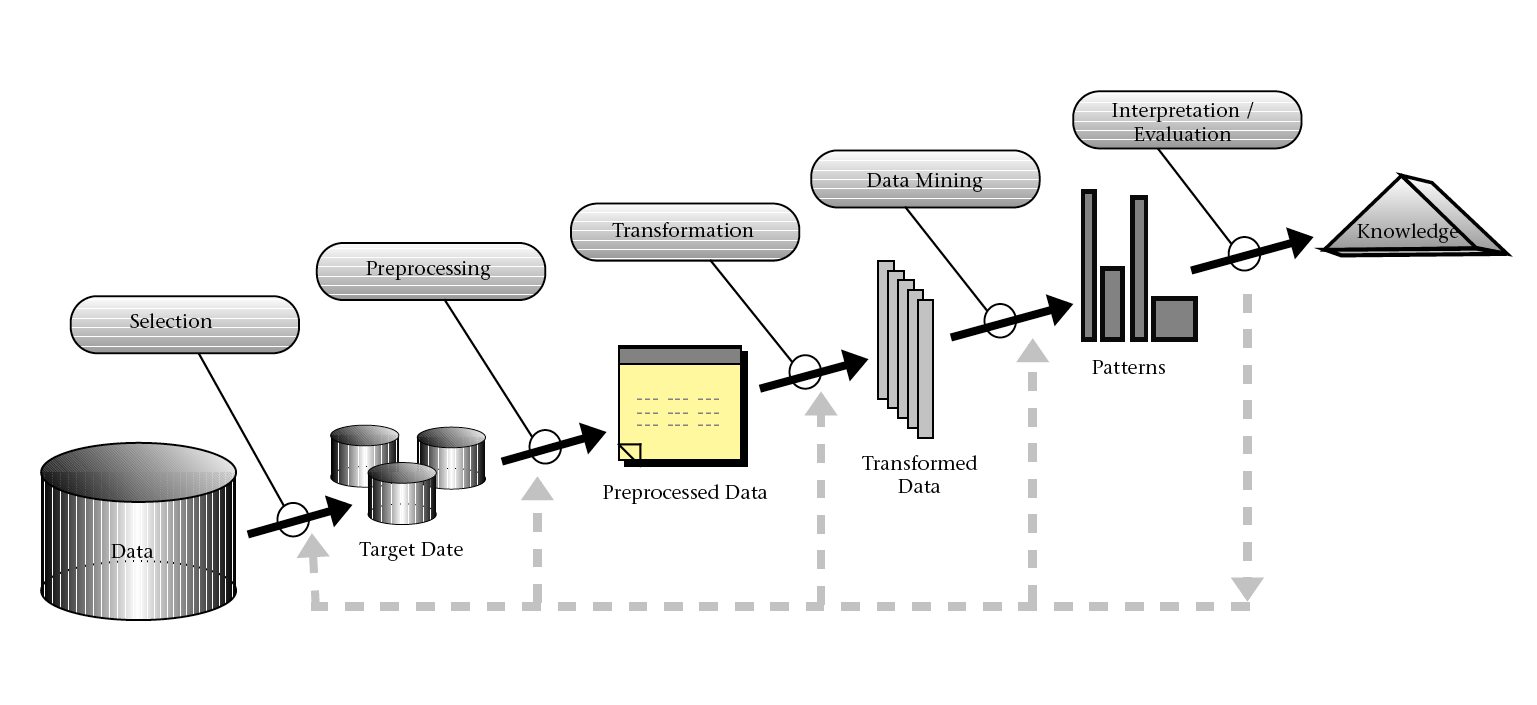
\includegraphics[width=5.5in,angle=0]{./sections/Fayyad96kdd-process.eps}
\end{center}
\caption{Overview of Knowledge Discovery System}
\label{fig:refSingleRobot1}
\end{figure}
The intrusion detection system should find specific kinds of abnomal traffic e.g. a denial of service (DoS) attack. 
It should check if these new sets of monitoring network traffic show similar properties as the orignal data or not as well. 
I construct the system similar to the knowledge discovery system \cite{fayyad96} because it is widely used among intrusion detection systems. 
A new approach to construct a pairwise similarity matrix is that it compares their probability in pairwise not its attributes directly. 
For this, the system includes gaussian mixture models for attributes and classes to calculate the probability for data point as I stated before. 
%The EM approach is used to fit those models and is guaranteed to converge to a local optimum on given input. 
With those components, we measure a score for each attributes, and those scores are weighted based on their importance in the dataset \cite{kayacik05}.
%to get 2D data where x-axis is a score for normal connection similarity and y-axis is a score for known abnormal connection similarity. 
The experiment suggests that such local optimum can effectively seperate different connections and most of unknown classes. 
%\begin{figure}[htb2]
%\begin{center}
%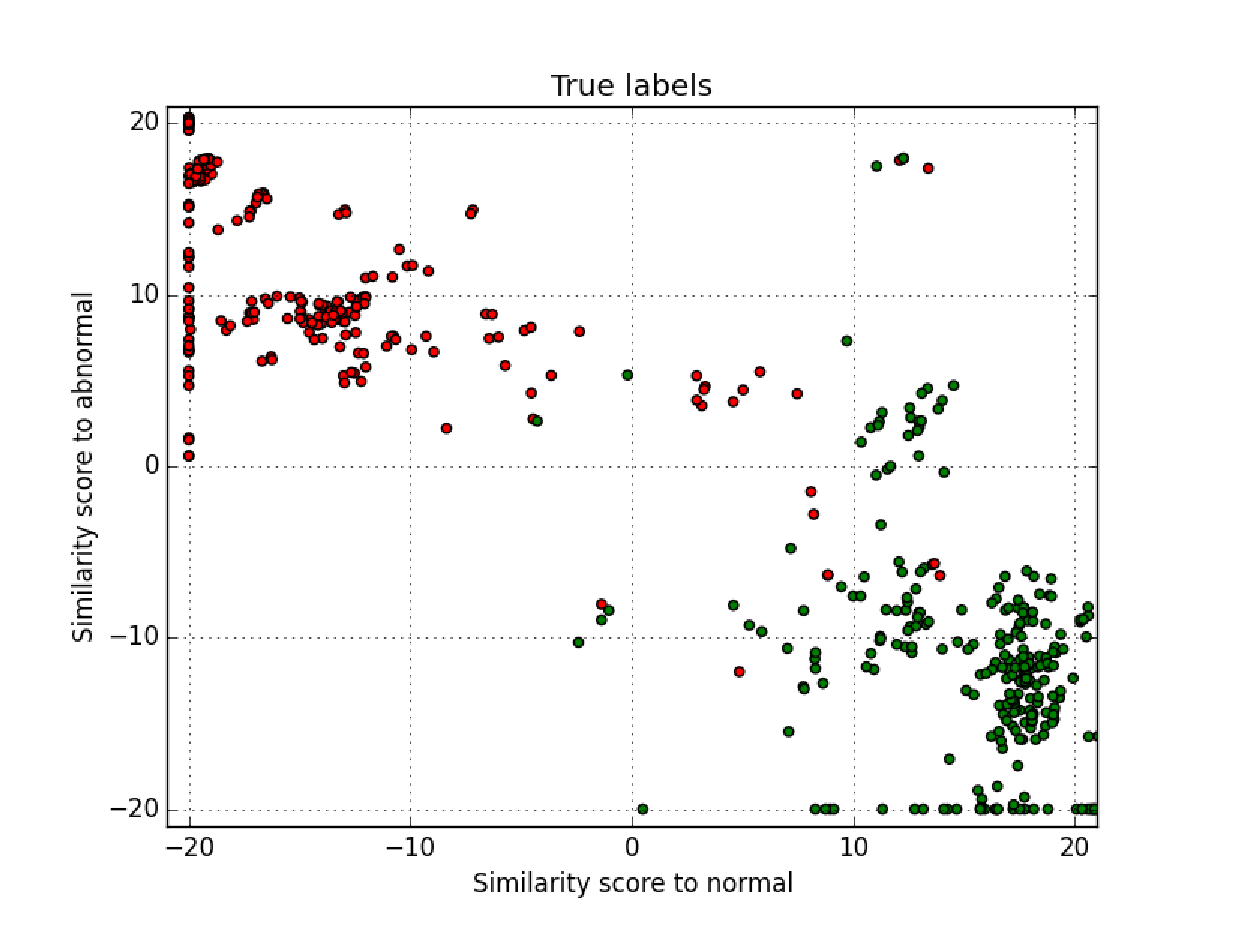
\includegraphics[width=3.5in,angle=0]{./sections/training20_only_true_.eps}
%\end{center}
%\caption{Similarity of normal and abnormal connections in training set.}
%% The left figure shows data points including known anomalies and the right known type of anomalies shows data points including unknown type of anomalies.} % I may show rest of data in appendix
%\label{fig:refSingleRobot1}
%\end{figure}

%In order for spectral anaysis, we need to make a sparse affinity matrix from transported data. 
%We can compute a sparse affinity matrix from a pairwise similarity matrix. 
After we have a pairwise similarity matrix, one way to convert similarity matrix to a sparse affinity matrix is that dealing with the affinities for $k$ nearest neighborhood, and set all other values for current data point to zero. 
I choose $k = 8$ because it is commonly used in spectral clustering approaches. 

% Altho require non-convex boundaries,
%\subsection{Computing affinity matrix}
%%The processing steps of the approach can be summerized as follows:
%%1) Training mixture model with training set containing records of both normal and anomalous connections.
%%2) The data are divided into different clusters for normal and anomalous connections using Spectral clustering algorithm.
%\subsubsection{Data pre-processing}
%\begin{itemize}
%\item categorical value to integer e.g.) service-type (ftp-data,http,etc).
%\item log of big number e.g.) duration, src-bytes.
%\end{itemize}
%\subsubsection{Affinity matrix computation}
%The data points are associated with each other by pairwise similarity.
%\begin{itemize}
%\item Construct similarity matrix with distance metric.
%\item Construct affinity matrix from similarity matrix with 8-nearest neighbors algorithm.
%\end{itemize}
%\subsection{Clustering}
%%\subsubsection{Number of clusters prediction}
%%Predict number of clusters based on the eigengap.
%%\subsubsection{Spectral clustering algorithm}
%%Normalized cut algorithm. \cite{jianbo00}
%%\subsubsection{Representative of clusters}
%%Clusters are represented by the mean and variance.
%\subsection{Detecting anomaly from clusters}
%%Distance based outlier detection is used.
%%\begin{itemize}
%%\item It do not require any prior knowledge.
%%\item k-nearest neighbor outlier detection algorithm. \cite{knorr00}
%%\end{itemize}

\subsection{Detecting Anomalies}
\label{subsec:detectinganomalies}
In this section, I describe how a sparse affinity matrix can be used to detect point and collective anomalies. 
In the following experiments, I divide experiments for known anomalies and unknown anomalies. 

\subsubsection{Known Anomalies}
We can see that trained normal and abnormal similarity functions are sensitive to known anomalies in the testset - their scores are similar to known anomalies and dissimilar to known normal connections. 
%normal and abnormal connections similarity are sensitive to known anomalies. 
It shows how much trained similarity functions capture the effects of an known anomalies. 
% The similarity coputed by mixture models gives similarity scores that are used to find k nearest neighborhood.
For most of classes, similarity of their points is very close to either known normal or abnormal connections. 
%In summary, all the class successfully detect known anomalies in spectral approach. 
However this approach does not work if the number of intrusions are insufficient because those classes are not well trained in mixture models, and data points tend to assigned to different clusters. 

\begin{figure}[htb2]
\begin{center}
\subfloat[Predicted labels]{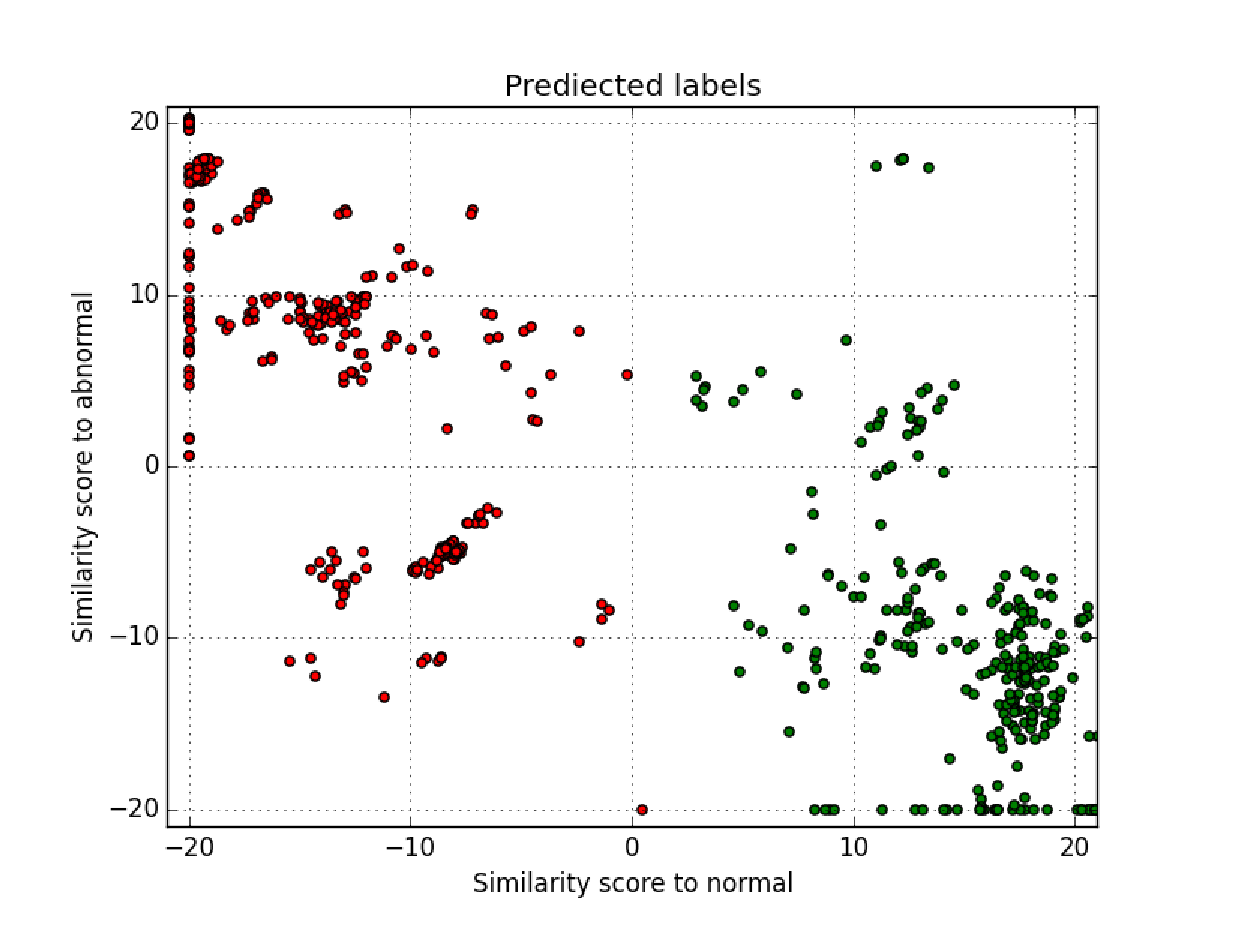
\includegraphics[width=3.0in,angle=0]{./sections/training20_test20_back_prediction_.eps}}
\subfloat[True labels]{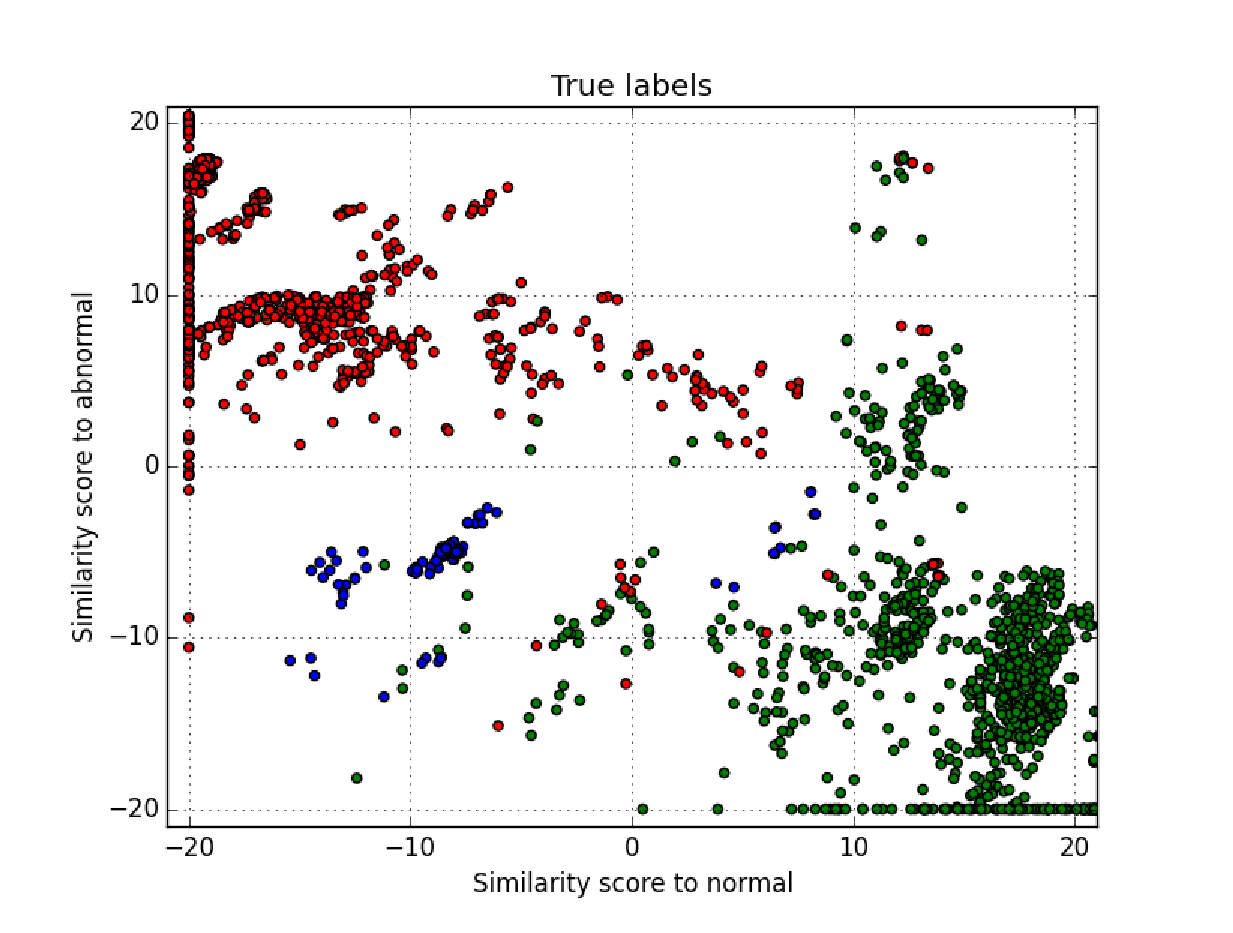
\includegraphics[width=3.0in,angle=0]{./sections/training20_test20_back_true_.eps}}
\end{center}
\caption{Anomaly detection for known anomalies. Red:Known and seen abnormal connections, Green:Known and seen normal connections, Blue:Intrusion "back" which is a known anomaly but in the testset.} % I may show rest of data in appendix
\label{fig:refSingleRobot1}

\end{figure}
\begin{table}[!ht]
\begin{center}
\begin{singlespace}
\scalebox{0.7}{
\begin{tabular}{| l | l | p{2cm} || l | l | p{2cm} |}
\hline
Type of Anomaly & Number & $\%$ correct & Type of Anomaly & Number & $\%$ correct \\
\hline
guess passwd & 1231 & 94.91 & ftp write & 3 & 66.66 \\
\hline
nmap & 73 & 85.71 & back & 359 & 98.03  \\
\hline
multihop & 18 & 100 & rootkit & 13 & 84.61  \\
\hline
pod & 41 & 100 & perl & 2 & 0  \\
\hline
ipsweep & 117 & 97.4 & teardrop & 12 & 100  \\
\hline
satan & 727 & 87.96 & loadmodule & 2 & 0  \\
\hline
buffer overflow & 20 & 90 & phf & 2 & 50  \\
\hline
warezmaster & 944 & 84 & imap & 1 & 100  \\
\hline
warezclient & 6 & 0 & land & 7 & 100  \\
\hline
neptune & 1579 & 89.23 & smurf & 627 & 95.33  \\
\hline
\end{tabular}
}
\end{singlespace}
\end{center}
\caption{Known anomalies detection rate}
\label{fig:refSingleRobot1}
\end{table}

%Result provides the sensitivity and the coverage of similarity measure that is effective. 
%All data point in testset for 21 known abnomal classes shows similar to known anomalies. 
%After it calcurate the similarity among data points 
%\begin{table}[h]
%\begin{center}
%\begin{tabular}{| l | l | l | p{5cm} |}
%\hline
%Type of Anomaly & Predicted normal & Predicted anormalies & $\%$ correct\\
%\hline
%True normal &  &  & \\
%\hline
%True anormalies &  &  & \\
%\hline
%\end{tabular}
%\end{center}
%\caption{Abnomal classes in NSL-KDD99}
%\label{fig:refSingleRobot1}
%\end{table}
% The detection rate for them are quite high. 
%
%\begin{figure}[htb2]
%\begin{center}
%\end{center}
%\caption{Clusters of connections including known anomalies. The x-axis shows the normal similarity scores and the y-axis shows the known abnormal similarity scores}
%\label{fig:refSingleRobot1}
%\end{figure}
\newpage
\subsubsection{Unknown Anomalies}
We see that normal and abnormal connection similarity are also sensitive to most of unknown anomaly. 
However, we have four classes that are similar to normal connections. 
Connection density similarity measure is sensitive in this type of anomaly if it is above its threshold. 

13 out of 17 unknown anomalies such as "processtable" class are similar to known anomalies. 
Therefore we can detect them with exactly same way what it have done to known anomalies. 
Those results are good as known anomalies. 

\begin{table}[h]
\begin{center}
\scalebox{0.7}{
\begin{tabular}{| l | l | p{2cm} || l | l | p{2cm} |}
\hline
Type of Anomaly & Number & $\%$ correct & Type of Anomaly & Number & $\%$ correct \\
\hline
processtable & 685 & 95.64 & named & 17 & 88  \\
\hline
udpstorm & 2 & 100 & sqlattack & 2 & 100  \\
\hline
ps & 15 & 100 & httptunnel & 133 & 81  \\
\hline
apache2 & 737 & 97.7 & saint & 309 & 98  \\
\hline
mscan & 996 & 97.42 & xterm & 13 & 100  \\
\hline
worm & 2 & 0 & xclock & 9 & 88.88  \\
\hline
xsnoop & 4 & 0  \\
\hline
\end{tabular}
}
\end{center}
\caption{Unknown anomalies that is similar to the known anomalies detection rate}
\label{fig:refSingleRobot1}
\end{table}

However 4 out of 17 are close to the normal connections in the trainingset. 
In that case, a cluster resulted by spectral clustering is denser than normal case can be detected by density based algorithm if we compare with mixture density generated by normal connections only. 
So with those prior knowledge we can use a spectral approach to find abnormal clusters which is originally classified as normal clusters. 

\begin{figure}[htb2]
\begin{center}
\subfloat[Predicted labels]{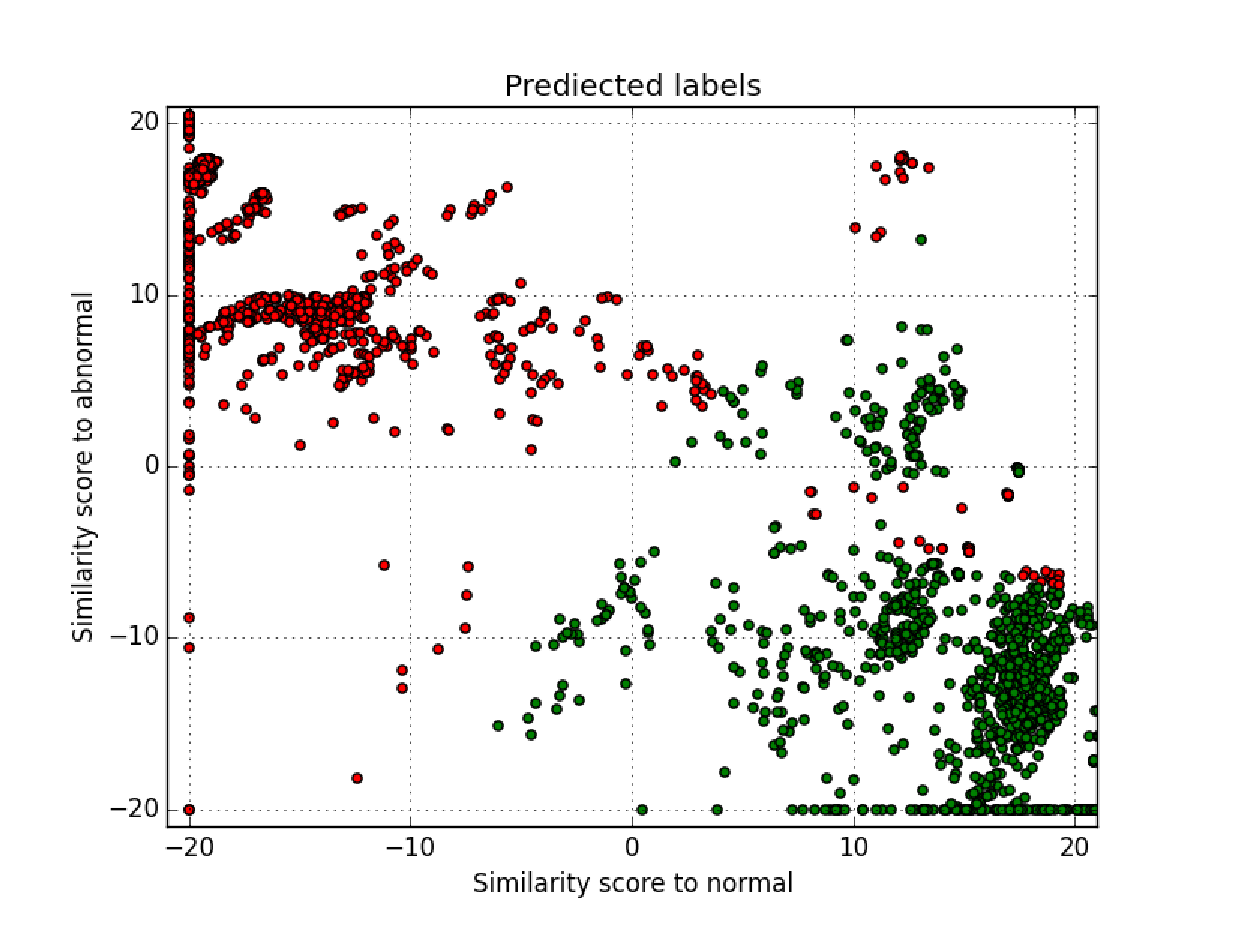
\includegraphics[width=2.0in,angle=0]{./sections/training20_test20_snmpguess_prediction_.eps}}
\subfloat[True labels]{\includegraphics[width=2.0in,angle=0]{./sections/training20_test20_snmpguess_true_.eps}}
\subfloat[Densities]{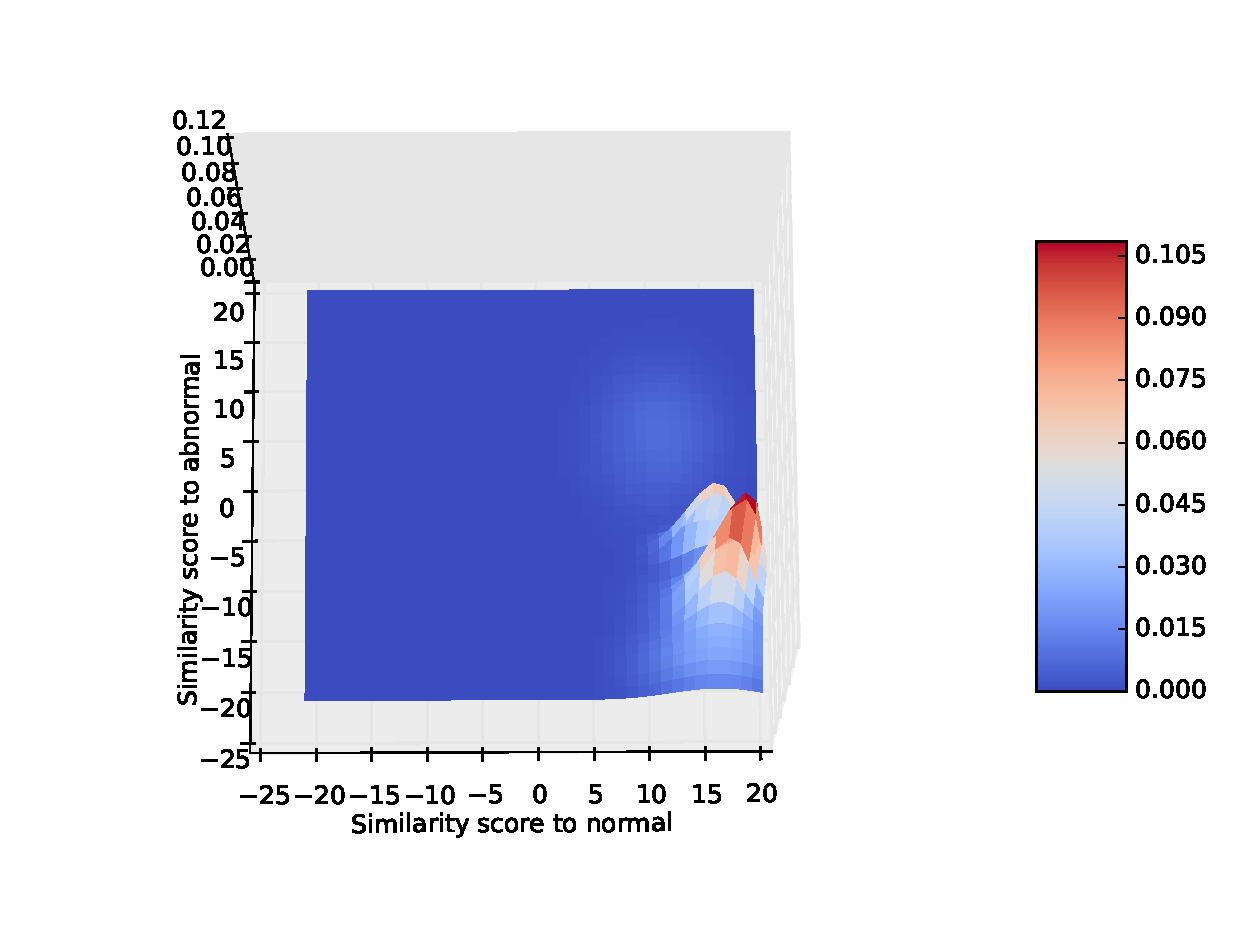
\includegraphics[width=2.0in,angle=0]{./sections/guess.eps}}
\end{center}
\caption{Density based intrusion detection result for unknown anomalies.  Red:Known and seen abnormal connections, Green:Known and seen normal connections, Blue:Intrusion "snmpguess" which is a unknown anomaly similar to normal connections.} % I may show rest of data in appendix
\label{fig:refSingleRobot1}
\end{figure}

The performance of density approach is not as good as previous one, and we can see that it is not able to detect "sendmail" class which is too few to form enough density. 
\begin{table}[h]
\begin{center}
\scalebox{0.7}{
\begin{tabular}{| l | l | p{2cm} || l | l | p{2cm} |}
\hline
Type of Anomaly & Number & $\%$ correct & Type of Anomaly & Number & $\%$correct \\
\hline
snmpguess & 331 & 55.5 & snmpgetattack & 178 & 58.9  \\
\hline
mailbomb & 293 & 24.7 & sendmail & 14 & 0  \\
\hline
\end{tabular}
}
\end{center}
\caption{Unknown anomalies that is similar to known normals detection rate}
\label{fig:refSingleRobot1}
\end{table}

%4 out of 17 are close to known normal connections. 
%We can not detect them with exactly same way what it have done to known anomalies since abnormal and normal connections are mixed together. 
%However we can differenciate with density approach after the spectral clustering. 
%Here is the result, and their performance is good. 
%\begin{table}[h]
%\begin{center}
%\begin{tabular}{| l | l | l | p{5cm} |}
%\hline
%Type of Anomaly & Predicted normal & Predicted anormalies & $\%$ correct\\
%\hline
%True normal &  &  & \\
%\hline
%True anormalies (close to A)&  &  & \\
%\hline
%True anormalies (close to N) &  &  & \\
%\hline
%\end{tabular}
%\end{center}
%\caption{Abnomal classes in NSL-KDD99}
%\label{fig:refSingleRobot1}
%\end{table}
%\begin{table}[h]
%\begin{center}
%\begin{tabular}{| l | l | p{5cm} |}
%\hline
%Type of Anomaly & Count & $ \%$ correct\\
%\hline
%guess passwd & 100 & 80 \\
%\hline
%ftp write & 3 & 66.66 \\
%\hline
%nmap & 73 & 85.71 \\
%\hline
%back & 100 & 98.03  \\
%\hline
%multihop & 18 & 100  \\
%\hline
%rootkit & 13 & 84.61  \\
%\hline
%pod & 41 & 100  \\
%\hline
%perl & 2 & 0  \\
%\hline
%ipsweep & 117 & 97.4  \\
%\hline
%teardrop & 12 & 100  \\
%\hline
%satan & 100 & 87.96  \\
%\hline
%loadmodule & 2 & 0  \\
%\hline
%buffer overflow & 20 & 90  \\
%\hline
%phf & 2 & 50  \\
%\hline
%warezmaster & 100 & 84  \\
%\hline
%imap & 1 & 100  \\
%\hline
%warezclient & 6 & 0  \\
%\hline
%land & 7 & 100  \\
%\hline
%neptune & 100 & 100  \\
%\hline
%smurf & 100 & 100  \\
%\hline
%processtable & 100 & 100  \\
%\hline
%named & 17 & 88  \\
%\hline
%udpstorm & 2 & 100  \\
%\hline
%snmpguess & 100 & 72  \\
%\hline
%sqlattack & 2 & 100  \\
%\hline
%ps & 15 & 100  \\
%\hline
%httptunnel & 100 & 81  \\
%\hline
%sendmail & 14 & 0  \\
%\hline
%snmpgetattack & 100 & 97  \\
%\hline
%apache2 & 100 & 100  \\
%\hline
%saint & 100 & 98  \\
%\hline
%mailbomb & 100 & 72  \\
%\hline
%mscan & 100 & 100  \\
%\hline
%xterm & 13 & 100  \\
%\hline
%worm & 2 & 0  \\
%\hline
%xclock & 9 & 88.88  \\
%\hline
%xsnoop & 4 & 0  \\
%\end{tabular}
%\end{center}
%\caption{Abnomal classes in NSL-KDD99}
%\label{fig:refSingleRobot1}
%\end{table}
